%%%%%%%%%%%%%%%%%%%%%%%%%%%%%%%%%%%%%%%%%%%%%%%%%%%%%%%%%%%%%%%%%%%%%%%%%%%%%%%%%%
%%% Platform Description
%%% Add sample data from cameras and lidar
%%% Section 1 : Hardware Overview
%%%		SubSection 1.1 : Pertinent Nao Statistics (and how things talk to each other)
%%% 	SubSection 1.2 : Pertinent Lidar Statistics
%%%		SubSection 1.3 : Design Requirements for Lidar Mount and Description
%%% Section 2 : Software Framework
%%%		SubSection 2.1 : NaoQi and qibuild Overview
%%% 	SubSection 2.2 : Custom Library Framework
%%%		SubSection 2.3 : User Operation
%%%
%%%%%%%%%%%%%%%%%%%%%%%%%%%%%%%%%%%%%%%%%%%%%%%%%%%%%%%%%%%%%%%%%%%%%%%%%%%%%%%%%%
\chapter{Platform}\label{ch:platform}

For this thesis we used the Nao as the mobile platform. Aldebaran makes him.
He's a cool little robot and he allows us to explore both things we wanted to 
look at which were navigation and gaiting. He's mobile, small, ``cost-effective''
and has a good API that we can use to do lower-level control of things when we want to, 
and abstract ourselves from it when we don't want to.
The small size means he's easy to work with.

There's definitely some more opening paragraph to be written here about the Nao.
Probably say something about why he's useful to investigate crawling.
No one's going to send Nao into a disaster zone or anything but he's not too
far off from robots that you would send in and we don't have to spend all the 
money or build a new lab to work with him. You can do lot's of simulations, 
but in the end you still have to test on a real robot.

While the Nao is cool and all, the sonar sensors just don't cut it for what we want to do.
Lucky, Nao comes with a USB port and uses x86 and linux so it's relatively
straightforward to add new things to him. Therefore, we added a better distance sensor.
Specifically we added the Hokuyo URG-04LX-UG01.
It's a good Lidar because it has a respectable range, good angular resolution,
``cost-effective'', and is kinda lightweight. Using this sensor we could do mapping 
if we wanted to which means this system is extensible to the broader challenges 
of the overall navigation problem such as SLAM\@. Using the Lidar we'll be able to 
get enough information to do the job we need to.

While it's easy to plug a USB cable into Nao's head, you still have to stick the Lidar somewhere.
Nao doesn't have mount points that make it easy to add new hardware.
Given that we have a nifty 3D printer (and I know Solidworks) we designed up a little suit of
armor for Nao with a big stick coming out of it that we could mount the Lidar to, above his head.
This works but the new dynamics destabilize Nao's default gait at certain speeds. 
This doesn't mess with the navigation algorithm, but to increase the speed this will have to be dealt with,
either by changing the rig or \ldots using the arms to counterbalance the new inertial forces as
part of the walking gait.

\section{Hardware Overview}
% Ok so, three pieces of hardware here, the Nao, the Lidar, and the mount.
% Technically, all you need is the Nao since it is a mobile base with distance sensors but the sonars
% don't do that great so we added the Lidar, and since there's no where to screw it down we designed a mount.

The hardware assembled for this platform can be divided into three major parts,
the Nao H25 Humanoid Platform, a Hokuyo URG-04LX-UG01 Lidar, and a custom 3D
printed assembly to mount the Lidar to the Nao.
The Nao acted as the mobile base and provided onboard sensing and computation. 
Its large number of degrees of freedom and humanoid configuration were amenable
to the exploration of crawling algorithms.
The Nao is also equipped with two color cameras for viewing the environment
and two sonars for measuring the range to objects.
% TODO: Maybe this should be restructured to highlight the roles the platform
% played in the Crawling and Navigation experiments, referenced by chapter.
In the navigation experiment, the forward facing camera was used to estimate
the pose to a goal object.
Though the two sonars can be used for obstacle
avoidance, previous experimentation showed they
were insufficient for navigation. This is because in a number of scenarios the
specular refections would cause confusing readings and the low angular
resolution would prevent the robot from walking through traversable apertures.
To supplement the Nao's sensor suite, the URG Lidar was mounted to the robot
to provide accurate, high resolution range data for use with navigation.
As the Nao does not have any external mounting points, a custom mount was
designed and constructed to allow the URG to be mounted to the Nao.


% Subsections about each hardware piece.
%\subsection{Goal Object}
Like many navigation algorithms, the one used in Chapter~\ref{ch:navigation}
requires the platform to have a goal location for which to traverse.
For these experiments, the goal location was provided to the robot by means
of a physical object that the robot could detect with its onboard camera.
The Nao API provides a simple ``red ball'' tracker that can be used to track
red objects via the onboard camera. It provides not only bearing information
but also range by assuming the red object has a width of $0.06 m$.

The goal was built as a $0.127 m$ wide red cube. 
This was affixed to the top of a wooden dowel, mounted to a heavy wooden base to 
allow it to be easily placed.
Figure~\ref{fig:red_cube1} shows a picture of the cube.
The dowel was approximately $0.6 m$ tall to allow the robot to see the cube
while minimizing the amount the head needs to pitch in order to keep 
the cube in view. Building the cube to be wider than the 
expected width allowed the target to be seen by the robot from longer distances. 
This longer range allowed for the construction of a larger arena as well as more 
robust tracking at shorter ranges.
The goal was built as a cube rather than a ball because during testing 
the tracking algorithm did not seem to be affected by the change in geometry 
and a cube was easier to construct. 

\begin{figure}
\centering
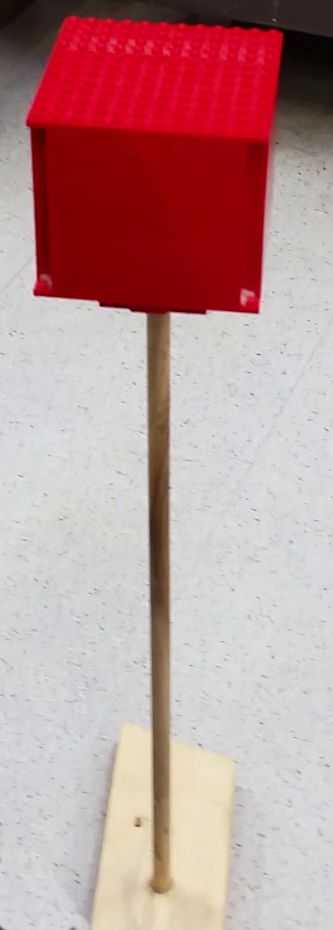
\includegraphics[height=0.4\textheight]{red_cube1.png}
\caption{Figure showing red cube the Nao tracked.}
\label{fig:red_cube1}
\end{figure}

%\subsection{Nao Hardware}
The Nao Humanoid Platform is made by Aldebaran Robotics. 
Figure~\ref{fig:crrl_nao_coronal1} shows a picture of the Nao at the
Control/Robotics Research Lab of NYU Polytechnic School of Engineering.
The robot weighs $5.4 kg$ and has a maximum forward velocity over flat
terrain of approximately $1 \frac{m}{s}$.
It has 25 degrees-of-freedom (DoF) embodied via a 2 DoF head, two 5 DoF legs,
two 5 DoF arms, two 1 DoF hands, and a 1 DoF hip.
Figure~\ref{fig:nao_joints1} shows a diagram locating each of the joints on
the robot.
% Sonars, joint sensors, cameras, foot sensors, IMU, bumpers and buttons.
Each joint has an absolute angular position encoder, while the feet each have
four force sensitive resistors to detect ground contact.
The head has two color cameras, one that faces forward and the other that faces
downward to get a view of the terrain. The chest contains a 2-axis gyroscope and
a 3-axis accelerometer for inertial measurement, and two sonar transmitter-receiver
pairs for measuring the range to obstacles.
Figure~\ref{fig:nao_features1} shows a diagram locating the various robot sensors,
including those not listed above.
% Battery life, weight, top speed (before and after Lidar), sonar ranges, camera angles and pixels,
The sonars have a minimum range of $0.25 m$ and a maximum range of $2.55 m$.
They have a resolution of $1 cm$ and detect any obstacle within a $60^\circ$
cone. The cameras have a $1.22 Mp$ resolution, $30 Hz$ frame rate,
a horizontal field-of-view of $60.9^\circ$, and a vertical field-of-view of
$47.6^\circ$.
% CPU type and speed, RAM, storage space, USB, Ethernet, WiFi.
The robot is equipped with a 1.6 GHz Intel\textsuperscript{\textregistered}
Atom\textsuperscript{TM} CPU, 1 GB of RAM, and 2 GB of Flash memory.
It also has Gigabit Ethernet, 802.11 b/g/n WiFi, and USB 2.0. 
Nao's operating system is called NAOqi OS which is a customized version of
Gentoo Linux. Being a Linux distribution, the robot can be easily accessed
using ssh, scp, and ftp. This allows familiar command line tools to be used
to script behavior and manage services.
The robot can be natively programmed using the provided C++ or Python API.

% Ok, now briefly review what's to come in the subsubsections.
The Nao is a very feature rich platform suitable for a variety of autonomous
applications. The following sections will review specific aspects of the robot
relevant to Chapters~\ref{ch:results_navigation} and~\ref{ch:results_crawling}.


\begin{figure}
\centering
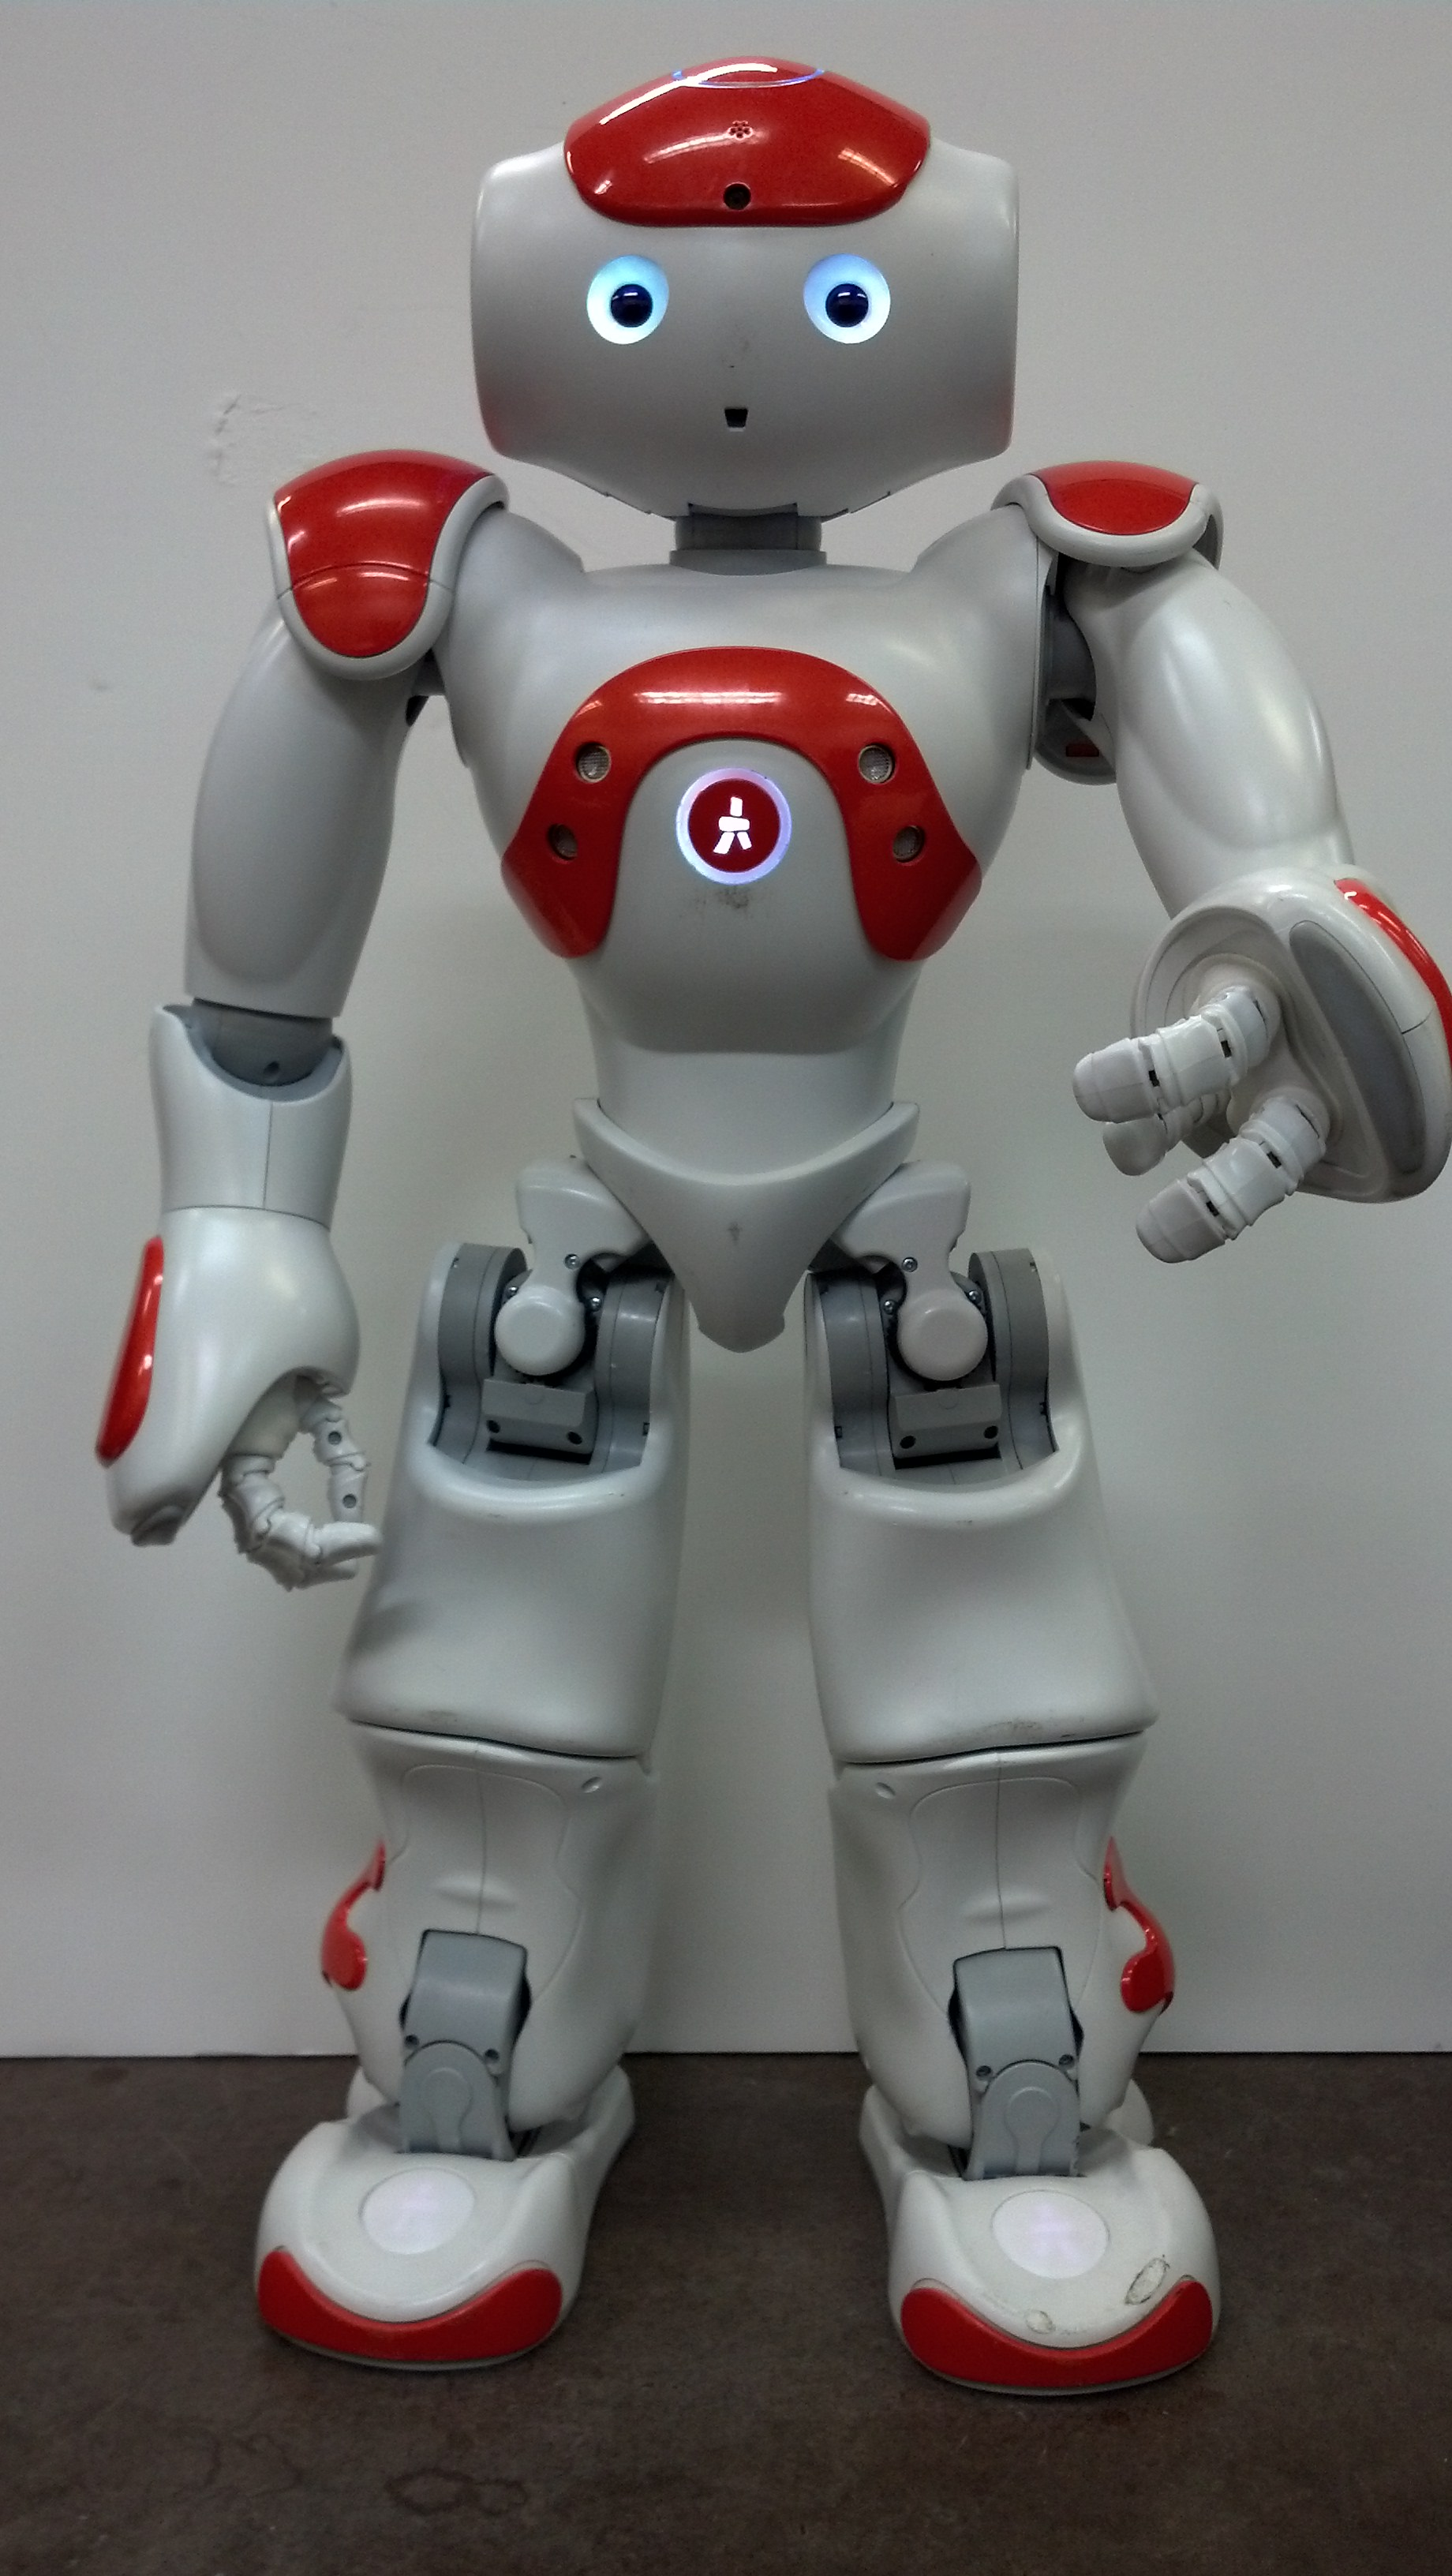
\includegraphics[height=0.4\textheight]{nao_coronal1.jpg}
\caption{Figure showing the Nao Humanoid Platform at the Control/Robotics
         Research Lab at NYU Polytechnic School of Engineering.}
\label{fig:crrl_nao_coronal1}
\end{figure}

\begin{figure}
\centering
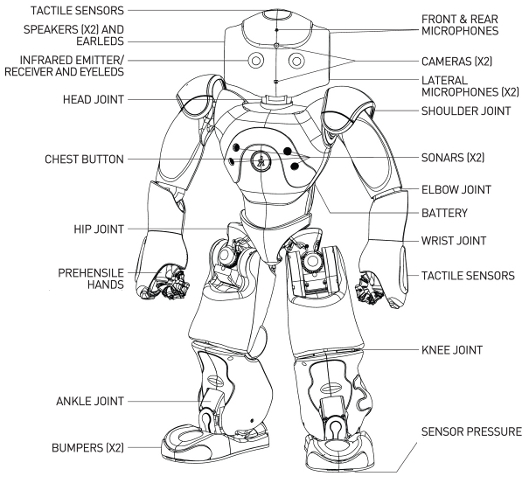
\includegraphics[width=0.4\textheight]{nao_diagrams/nao_h25_pres.png}
\caption{Figure locating the various features on the robot.}
\label{fig:nao_features1}
\end{figure}

\begin{figure}
\centering
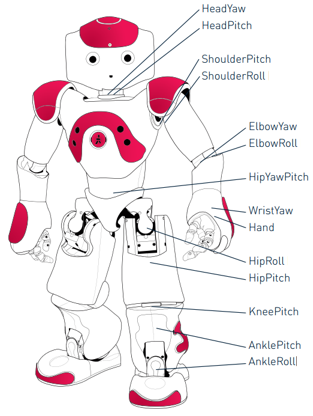
\includegraphics[height=0.4\textheight]{nao_diagrams/hardware_motortype_h25V5.png}
\caption{Figure indicating the various joint locations and their names.}
\label{fig:nao_joints1}
\end{figure}

\FloatBarrier

\subsubsection{Frame Definitions}
The NAOqi API defines three frames that can be seen in Figure~\ref{fig:nao_frames1}.
They are FRAME\_TORSO, FRAME\_ROBOT, and FRAME\_WORLD\@.
The first two frames, FRAME\_TORSO and FRAME\_ROBOT, are rigidly
attached to the robot, while FRAME\_WORLD is an inertial frame initialized
when the robot first starts.

\paragraph{FRAME\_TORSO} 
is a frame rigidly attached to the torso of the Nao. The positive Z-axis points
up through the head of the robot, while the positive X-axis points forwards.
It is useful for referencing different parts of the robot such and joint frames
and manipulation targets relative to the robot.
The frame origin along the X and Y directions is in the geometric center
of the torso, while Figure~\ref{fig:nao_link_lengths1} shows its Z location on
the torso as the point that the neck and hip offsets are referenced with
respect to.

\paragraph{FRAME\_ROBOT}
is a frame whose origin is between the feet of the robot. It's positive Z-axis
always points upwards and positive X-axis always points forwards. It is useful
when specifying navigation targets, relative to the Nao's current pose.

\paragraph{FRAME\_WORLD}
is a frame that is coincident with FRAME\_ROBOT when the Nao is started,
and remains static for the life of the run. It is useful for specifying navigation
and manipulation targets in a global coordinate sense.

\begin{figure}[H]
\centering
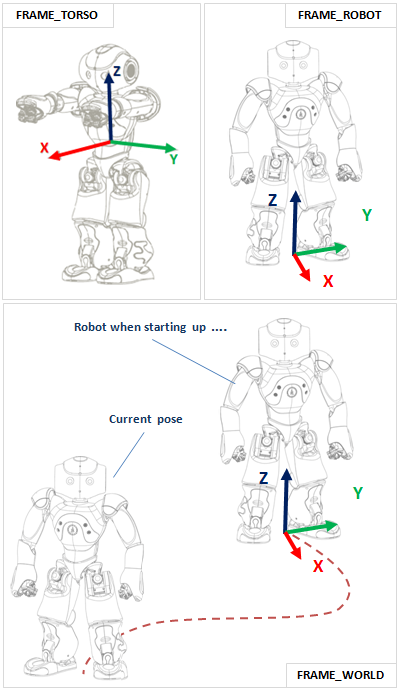
\includegraphics[height=0.75\textheight]{nao_diagrams/frame_definition_combo.png}
\caption{Nao frames.}
\label{fig:nao_frames1}
\end{figure}

Orientation targets for the Nao are commonly expressed using Tait-Bryan angles,
more commonly known as roll, pitch, and yaw. As can be seen in
Figure~\ref{fig:nao_rpy_def1}, yaw is expressed as rotation about the Z-axis,
roll is about the X-axis, and pitch is about the Y-axis.
When the robot is being referenced from the FRAME\_TORSO and is
initialized in the StandZero posture referenced in the proceeding section,
the naming conventions of the joints become clear. All joints whose axis
are parallel to the torso frame Y-axis are postfixed with the word ``Pitch'',
those parallel to the Z-axis are postfixed with the word ``Yaw'', and X-axis
with ``Roll''. The only exception to this rule is the ganged pelvis joint
axis. Each side of this degree of freedom rotates along a vector that is
in the plane formed by the torso Z-Y axes and is therefore postfixed with the
term ``YawPitch''.

\begin{figure}
\centerline{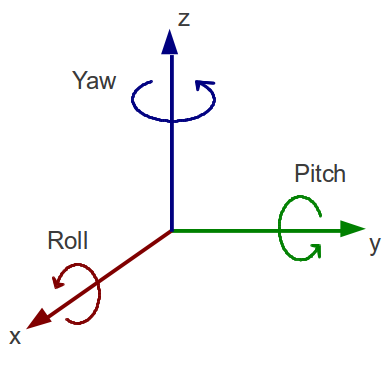
\includegraphics[width=0.5\textwidth]{nao_diagrams/rollPitchYaw.png}
}
\caption{Definition of roll pitch and yaw.}
\label{fig:nao_rpy_def1}
\end{figure}


\subsubsection{Links and Joints}
The Nao H25 is a bipedal platform with two legs, two arms, and an articulate
head. Each arm is composed of 5 joints and 3 non-zero length links, as are 
the legs, and the head is composed of 2 joints. There are also three fingers
per hand and two feet. Detailed measurements and specifications on the
Nao H25 can be found on the Aldebaran Website~\cite{nao_docs_h25}.
We will review a few relevant characteristics of the robot below.

\paragraph{Links}
Figure~\ref{fig:nao_link_lengths1} shows some of the large scale link lengths
of the Nao H25. The hip and neck Z offsets are measured with respect to
FRAME\_TORSO, as are the shoulder and hip Y offsets. The thigh and tibia lengths
are each roughly $100 mm$. Their total is $202.8 mm$. The neck and hip offsets
sum to $211.5$, making the torso approximately the same length as the legs.
The humerus of the robot is again nearly $100 mm$ though the forearm to the wrist
is half as long. The wrist to the hand is again about half as long as the
humerus, meaning in total, the arms are about as long and the legs.

\begin{figure}
\centerline{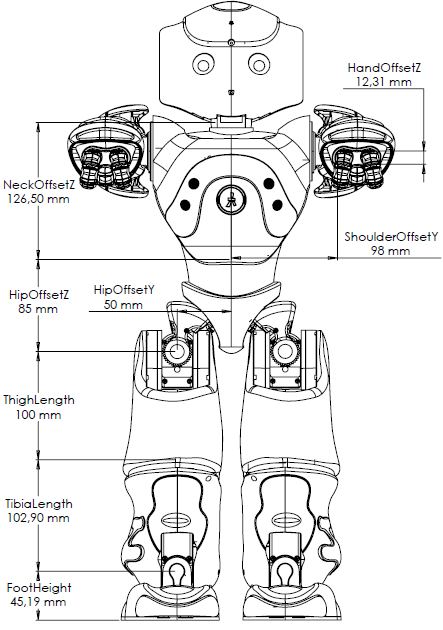
\includegraphics[width=0.45\textwidth]{nao_diagrams/hardware_lengthfront_3.3.png}
            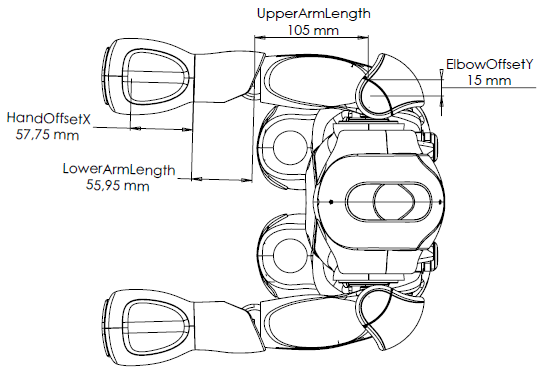
\includegraphics[width=0.55\textwidth]{nao_diagrams/hardware_lengthup_3.3.png}
}
\caption{Nao link lengths.}
\label{fig:nao_link_lengths1}
\end{figure}

\paragraph{Joints}
This needs to be said.
In the below diagrams, the green line represents the nominal zero, the blue line
is the min angle, and the red line is the max angle
\begin{figure}
\centering
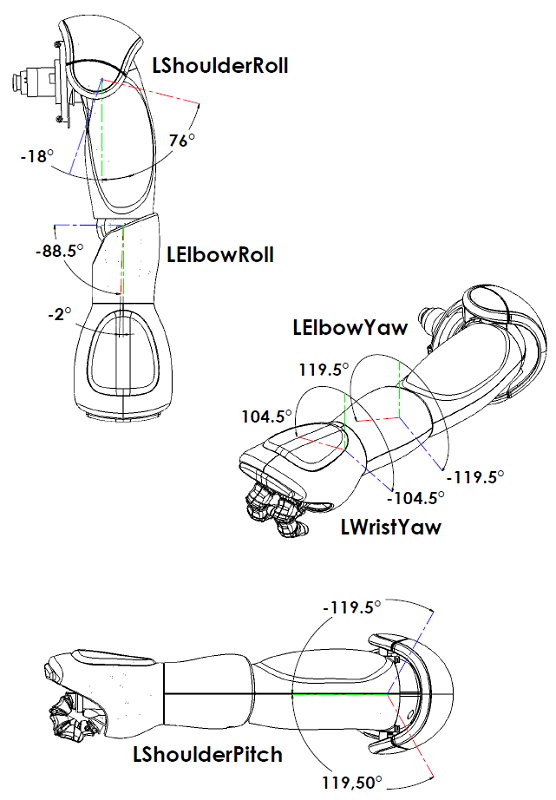
\includegraphics[width=\textwidth]{nao_diagrams/hardware_larmjoint_3.3_corr1.png}
\caption{Figure showing left arm}
\label{fig:nao_arm_joints_left1}
\end{figure}

\begin{figure}
\centering
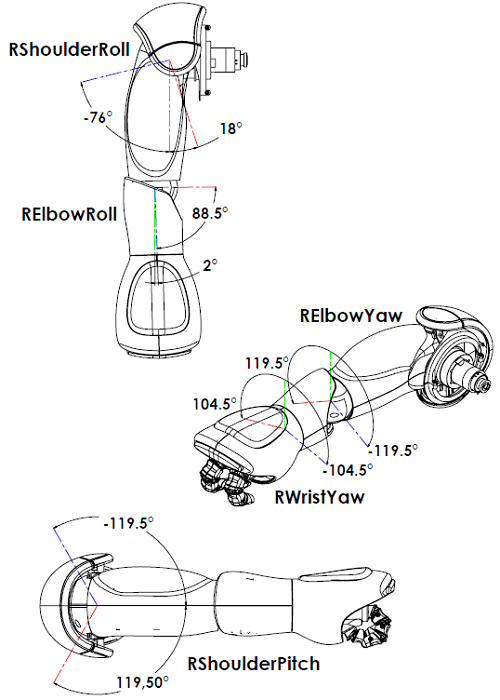
\includegraphics[width=\textwidth]{nao_diagrams/hardware_rarmjoint_3.3.png}
\caption{Figure showing right arm}
\label{fig:nao_arm_joints_right1}
\end{figure}

\begin{figure}
\centering
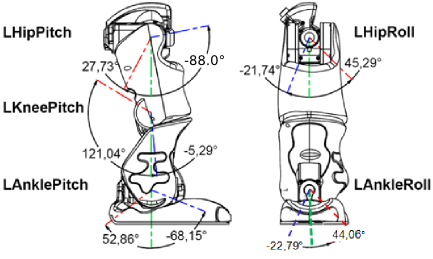
\includegraphics[width=\textwidth]{nao_diagrams/hardware_llegjoint.png}
\caption{Figure showing left leg}
\label{fig:nao_leg_joints_left1}
\end{figure}

\begin{figure}
\centering
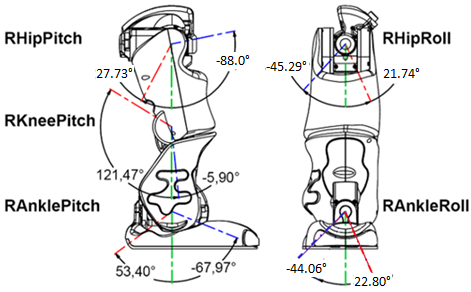
\includegraphics[width=\textwidth]{nao_diagrams/hardware_rlegjoint.png}
\caption{Figure showing right leg}
\label{fig:nao_leg_joints_right1}
\end{figure}

\begin{figure}
\centering
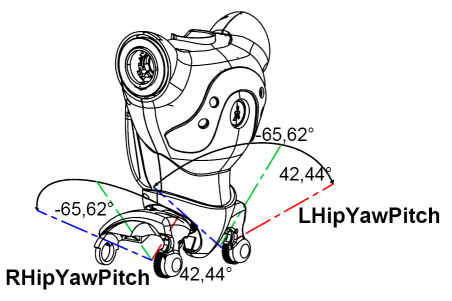
\includegraphics[width=\textwidth]{nao_diagrams/hardware_pelvisjoint.png}
\caption{Figure showing hip yaw-pitch}
\label{fig:nao_hip_yawpitch1}
\end{figure}

\paragraph{Arm Symmetry}
Need diagram showing arm symmetry for crawl results. 

\begin{figure}
\centering
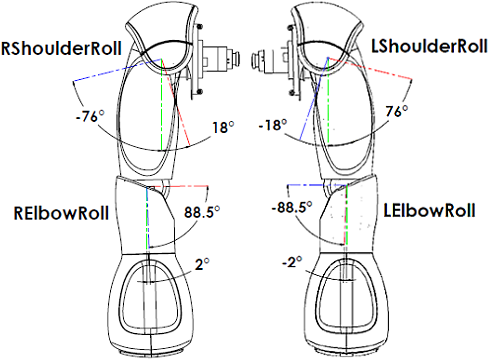
\includegraphics[width=\textwidth]{hardware_r_and_l_armjoint_corr1.png}
\caption{Figure showing arm joints and how they are a reflection.}
\label{fig:nao_arm_joints_reflect1}
\end{figure}

\FloatBarrier

\subsubsection{Joint Torques}
% Motor torques. (Important for Chapter~\ref{ch:crawl_gait})
Talking about the joint motor torques, tables, gearboxes, blah.

\subsubsection{Postures}
Talking about the different postures of the robot.

\begin{figure}
\centerline{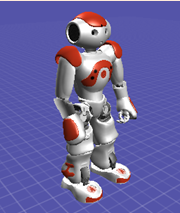
\includegraphics[width=0.33\textwidth]{posture/posture_stand.png}
            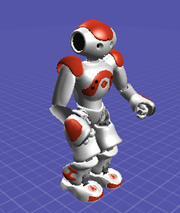
\includegraphics[width=0.33\textwidth]{posture/posture_standinit.png}
            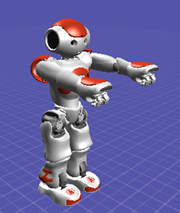
\includegraphics[width=0.33\textwidth]{posture/posture_standzero.png}
}
\vspace*{0.05in}
\centerline{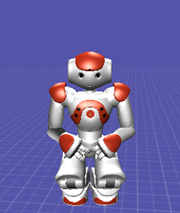
\includegraphics[width=0.33\textwidth]{posture/posture_crouch.png}
            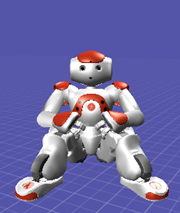
\includegraphics[width=0.33\textwidth]{posture/posture_sit.png}
            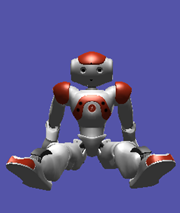
\includegraphics[width=0.33\textwidth]{posture/posture_sitrelax.png}
}
\vspace*{0.05in}
\centerline{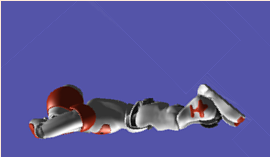
\includegraphics[width=0.5\textwidth]{posture/posture_lyingbelly.png}
            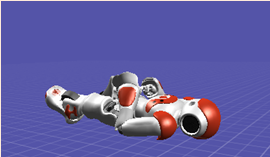
\includegraphics[width=0.5\textwidth]{posture/posture_lyingback.png}
}
\caption{Figure showing postures.}
\label{fig:nao_postures1}
\end{figure}

%\subsection{Lidar Hardware}
The sensor used to detect environmental obstacles was a Hokuyo
URG-04LX-UG01, which can be seen in Figure~\ref{fig:lidar_top1}. 
The URG is a 2D scanning laser rangefinder, more commonly known as
a Lidar. Lidar is a portmanteau for \textit{Li}ght \textit{D}etection 
\textit{a}nd \textit{R}anging and operates using principles similar 
to Radar and Sonar. 2D Lidars provide a number of discrete range measurements
along a plane. This effectively gives a ``top-down'' or ``blue-print''
style view of an environment.
This, when mounted to a robot, allows the detection of objects in one plane of
the environment so that the robot can avoid or plan a path around them.

\begin{figure}
\centering
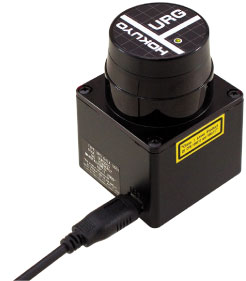
\includegraphics[height=0.3\textheight]{hokuyo/urg_04lx_ug01_top.jpg}
\caption{Photograph of the URG-04LX-UG01 Lidar. It is shown
         with a USB cable plugged in, which is the method of powering
         and retrieving data from the Lidar.}
\label{fig:lidar_top1}
\end{figure}

2D scanning Lidars such as the URG, sense the environment by emitting a laser
beam and measuring the time it takes for the emitted photons to return to the sensor.
This time is used to compute the range to the obstacle that the beam encountered.
Commonly, photons are not actually timed, but rather the phase difference of the
emitted light is used to estimate the time.
Following this measurement, the laser is then mechanically rotated to another 
angular position to take another reading. The process is repeated through the 
entire scanning angle of the sensor, and the set of range-angle pairs is 
considered ``one scan''. The URG uses a spinning mirror to rotate the beam, while
other sensors rotate the entire laser assembly.
An example of the data returned from the URG can be seen in Figure~\ref{fig:lidar_scan1}.
The URG was placed in a hall with a doorway to its left.

\begin{figure}
\centering
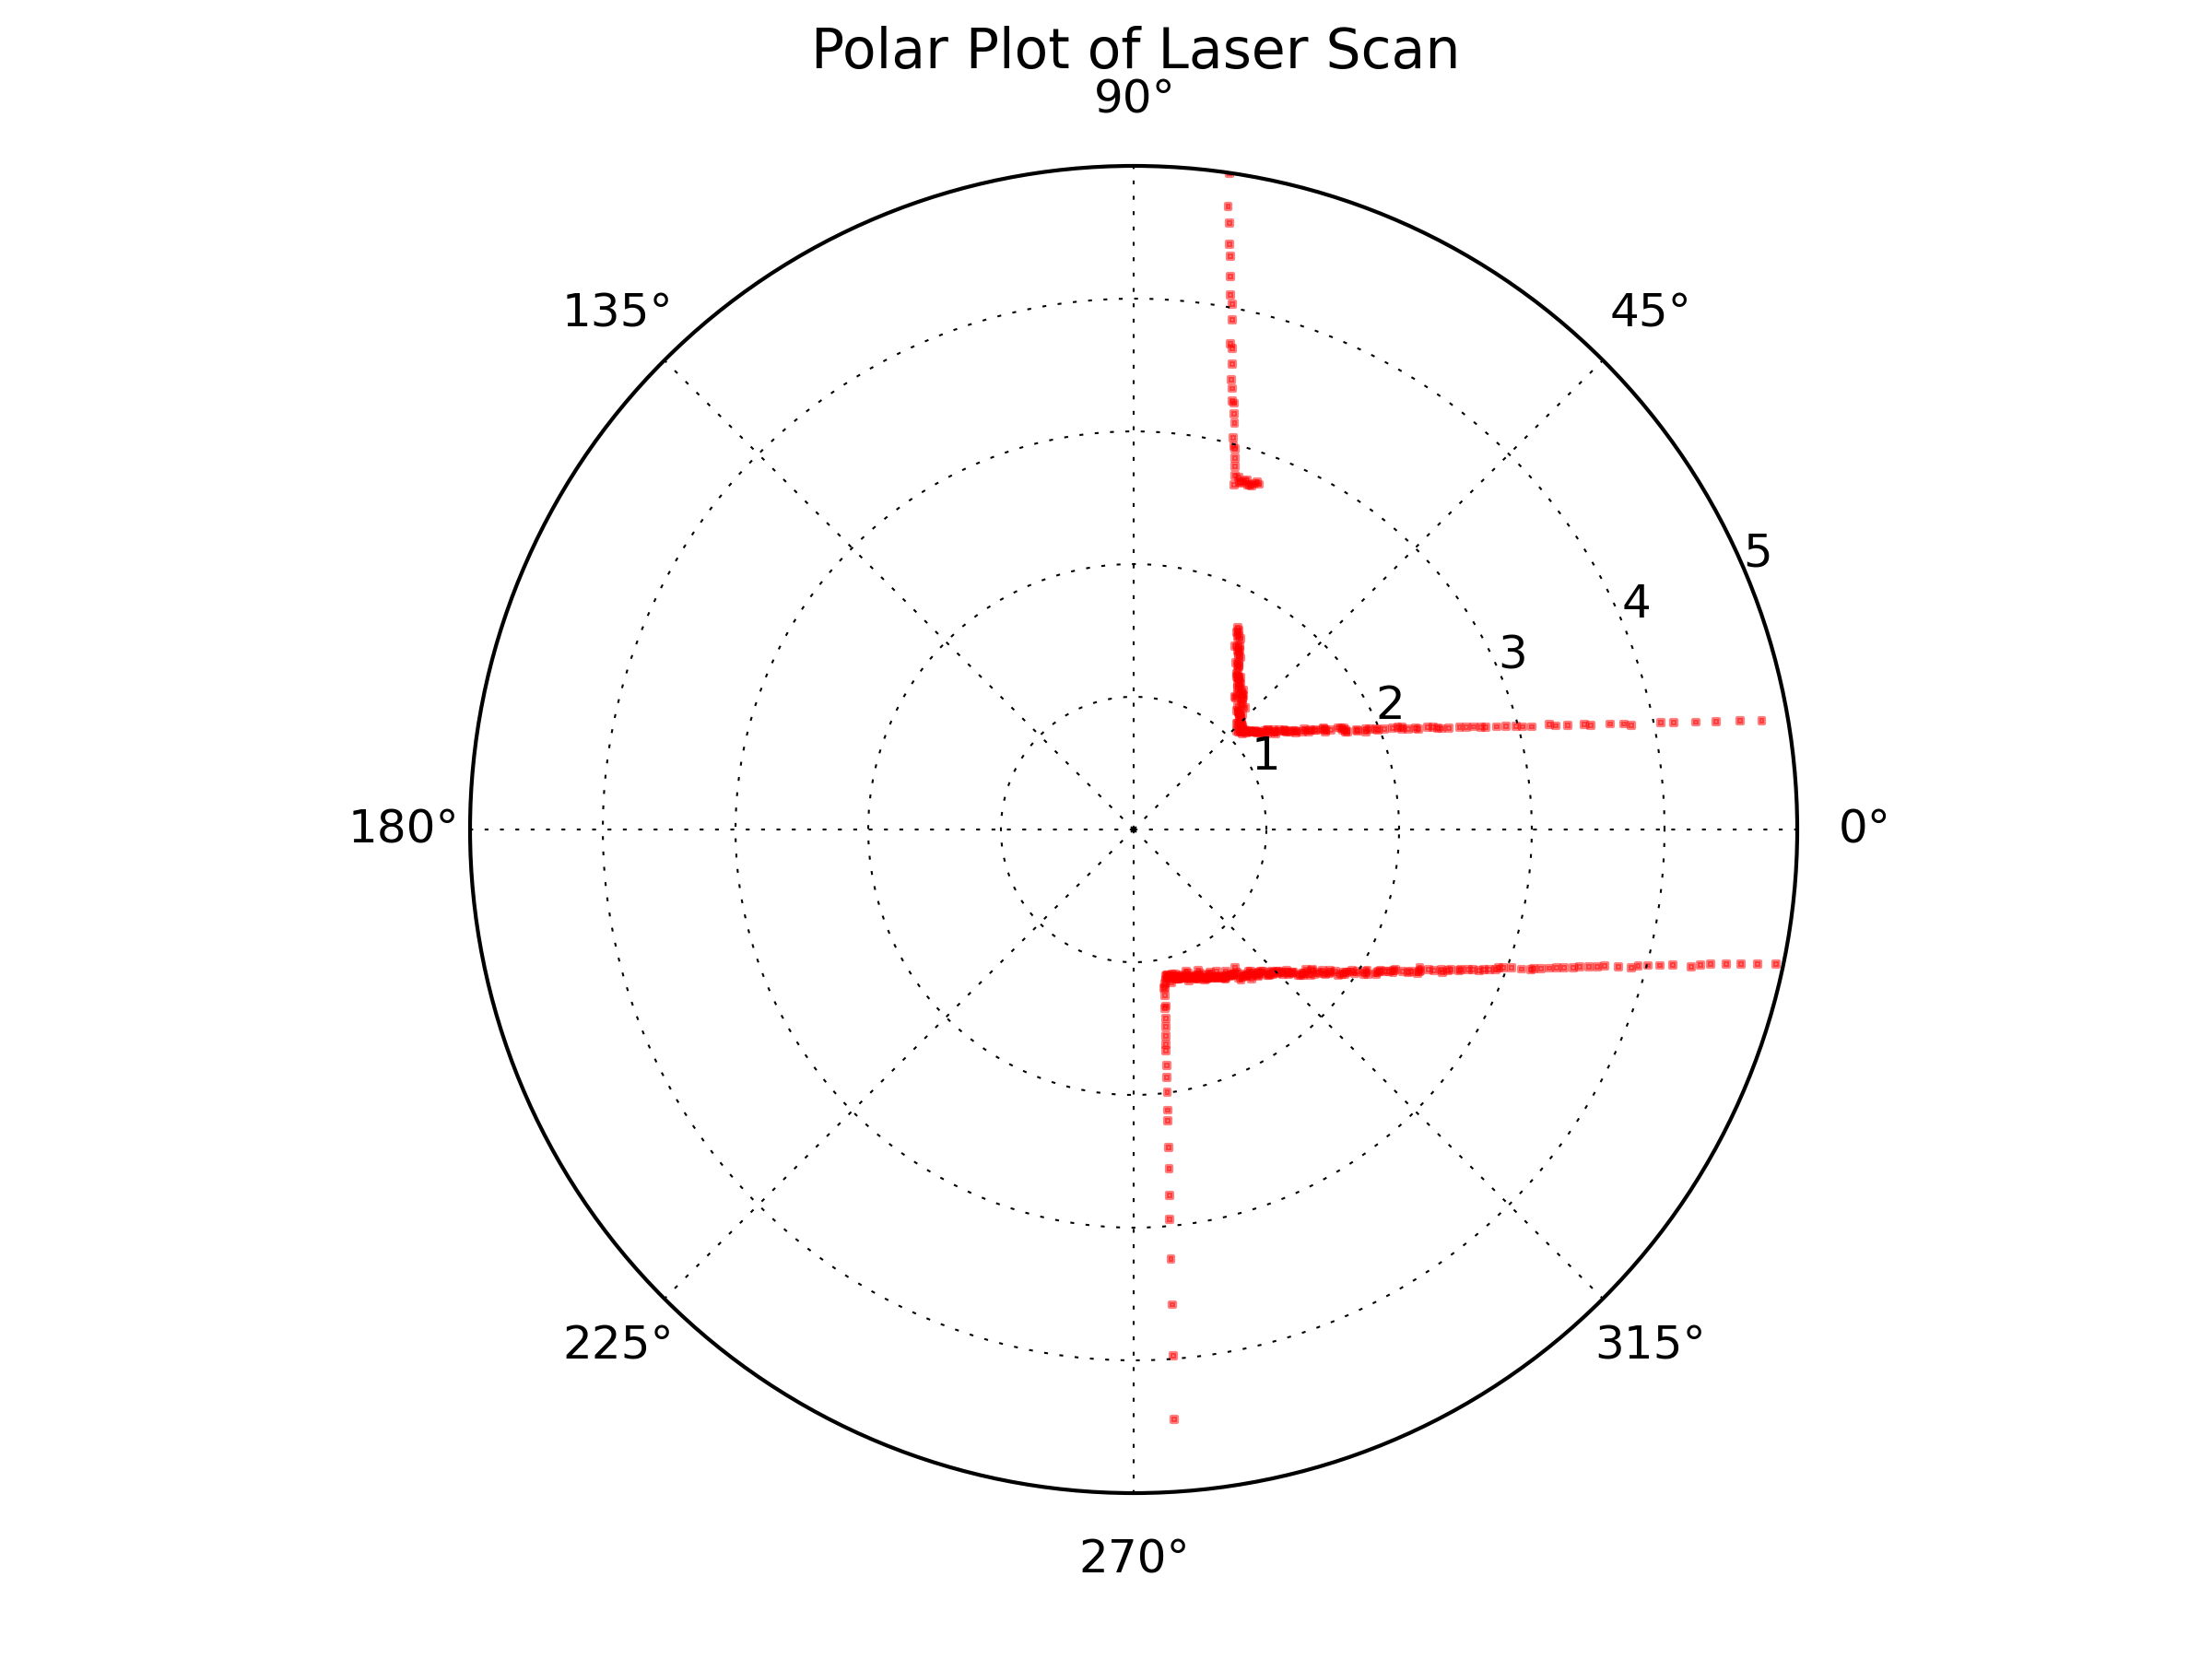
\includegraphics[height=0.4\textheight]{laser_scan_msg2.yaml_1.png}
\caption{Scan from the URG\@.
         The sensor is in the center of the figure.
         The radius of the figure is limited to 5 meters, which is 1 meter 
         greater than the maximum rated range of the sensor. While the unit will
         still provide data at this range, its accuracy is unrated.
         In this scan, the sensor is facing a hall, with a doorway to its left.}
\label{fig:lidar_scan1}
\end{figure}

The URG is a good choice for these experiments due to its lightweight and small
dimensions. This allows it to be easily mounted to the Nao Humanoid while
respecting the payload capacity of the robot. It has a wide scan angle, high
angular resolution, and a good range for this application. A high angular
resolution allows the robot to detect narrow obstacles that might obstruct the
robot's path, yet unlike sonar, provide detailed information about unobstructed
areas the robot can traverse. While the URG is rated for indoor use only, this
is sufficient for our application as the Nao is not often used in outdoor 
situations. Lastly, the sensor can be operated through a single USB port,
sourcing power from and providing data to the robot. This means no additional hardware is 
necessary for the Nao to make use of the sensor, as a USB port is available
in the back of the robot's head.
Figure~\ref{fig:lidar_diagram1} shows a mechanical drawing of the sensor, while
Table~\ref{tab:lidar_params1} lists some of the relevant specifications of the
URG.

\begin{table}
\centering
\begin{tabulary}{\textwidth}{|l||l|r|r|r|l|}
\hline
\textbf{Properties}& \textbf{Condition}         & \textbf{Min} & \textbf{Typ} & \textbf{Max} & \textbf{Units} \\	\hline\hline
\textbf{Scanner}   &                            &              &              &              &                \\	\hline
View Angle 	       &                            &              & 240          &              & degrees        \\	\hline
Angular Resolution &                            &              & 0.36         &              & degrees        \\	\hline
Range 	           &                            & 20           &              & 4000         & mm             \\	\hline 
Linear Resolution  &                            &              & 1            &              & mm             \\	\hline 
Accuracy           & Distance: 20 mm to 1000 mm &              & $\pm$ 30     &              & mm             \\	\hline 
        	       & Distance: 20 mm to 4000 mm &              & $\pm$ 3      &              & \%             \\	\hline \hline 
\textbf{Mechanical}&                            &              &              &              &                \\	\hline
Update Rate	       &                            &              & 100          &              & ms/scan        \\	\hline 
Weight             &                            &              & 160          &              & g              \\	\hline 
Width              &                            &              & 50           &              & mm             \\	\hline 
Length             &                            &              & 50           &              & mm             \\	\hline 
Height             &                            &              & 70           &              & mm             \\	\hline \hline
\textbf{Electrical}&                            &              &              &              &                \\	\hline 
Voltage Rating     &                            & 4.75         & 5.0          & 5.25         & V              \\	\hline 
Current Draw       &                            &              & 500          & 800          & mA             \\	\hline 
\end{tabulary} 
\caption{This table contains various specifications of the Hokuyo URG-04LX-UG01.
         These values were taken from the datasheet of the Lidar, which can be found here~\cite{urg_specs}.}
\label{tab:lidar_params1}
\end{table}

\begin{figure}
\centering
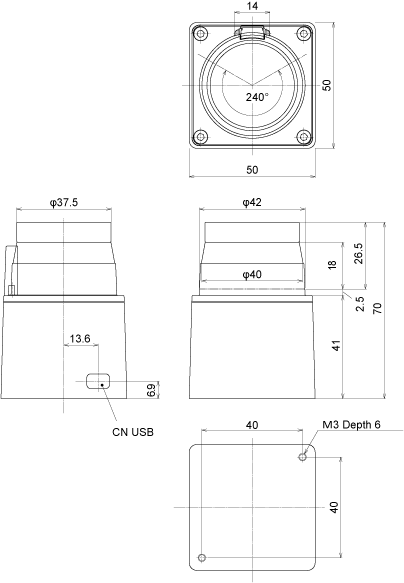
\includegraphics[height=0.3\textheight]{hokuyo/urg_04lx_ug01_ed.png}
\caption{Mechanical drawing of the URG-04LX-UG01.
         The compact size of the URG makes it easy to mount to the Nao.}
\label{fig:lidar_diagram1}
\end{figure}

\subsection{Lidar Mount}
% Design reqs: needed to rigidly attach to Nao for data transformation purposes, needed to see forward,
% lightweight, Nao needed to be able to move his head while wearing it,
% needed to be able to use the sonars (just in case).
In order to attach the URG Lidar to the Nao a custom Lidar mount was built.
The mount needed to hold the Lidar such that obstacles in front of the robot
could be sensed. The mount needed to be lightweight, rigidly attached, and allow
the robot to move its head to track the red cube. It should also not inhibit
the use of the sonars, in the event that the sonars are used in the future.

% Mounting it to the head seemed like it was going to be tough, so a vest was designed.
% Straps and foam seemed like they'd hold well enough. In fact they hold so well I can lift Nao up by the mount.
% The mount was made from PLA, 3D printer, foam, velcro straps.
As the Nao is not equipped with any mounting points, the Lidar mount was 
designed as a tray mounted to the front of the robot at waist-height, attached
using straps. The rigid parts were manufactured out of PLA plastic using a 3D
printer. The rigid parts that would contact the robot were padded with foam to
create a surface that would conform to the Nao's body and hold securely.
Figure~\ref{fig:nao_lidar_mount_nao_dimetric1} shows a CAD model of the finished
assembly.
A picture of the assembly mounted to the robot can be seen in
Figure~\ref{fig:nao_lidar_mount_picture1}.

\begin{figure}
\centering
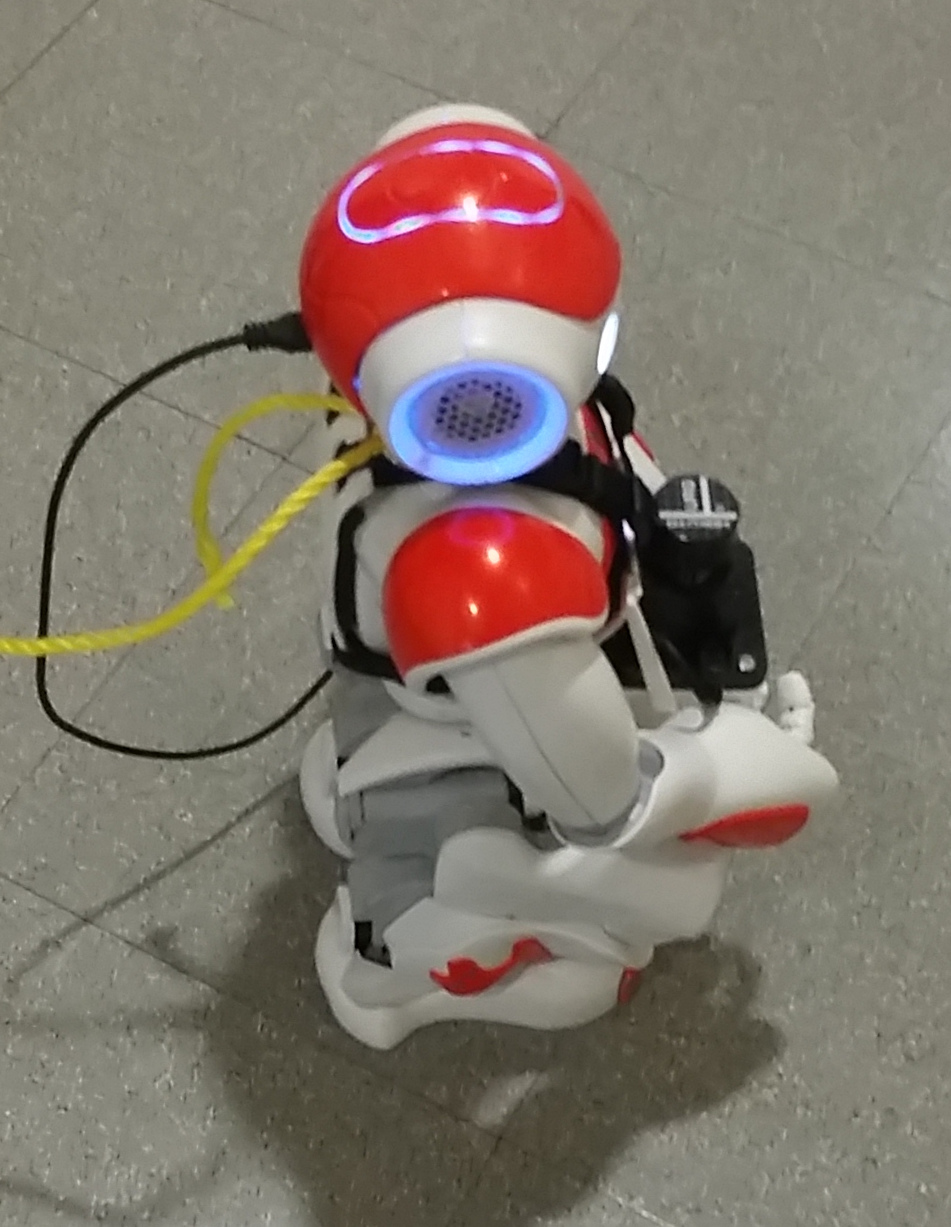
\includegraphics[height=0.4\textheight]{backpack/nao_with_mount2.jpg}
\caption{Figure showing a photograph of the URG mounted to the Nao using the
         custom Lidar mount.}
\label{fig:nao_lidar_mount_picture1}
\end{figure}

\begin{figure}
\centering
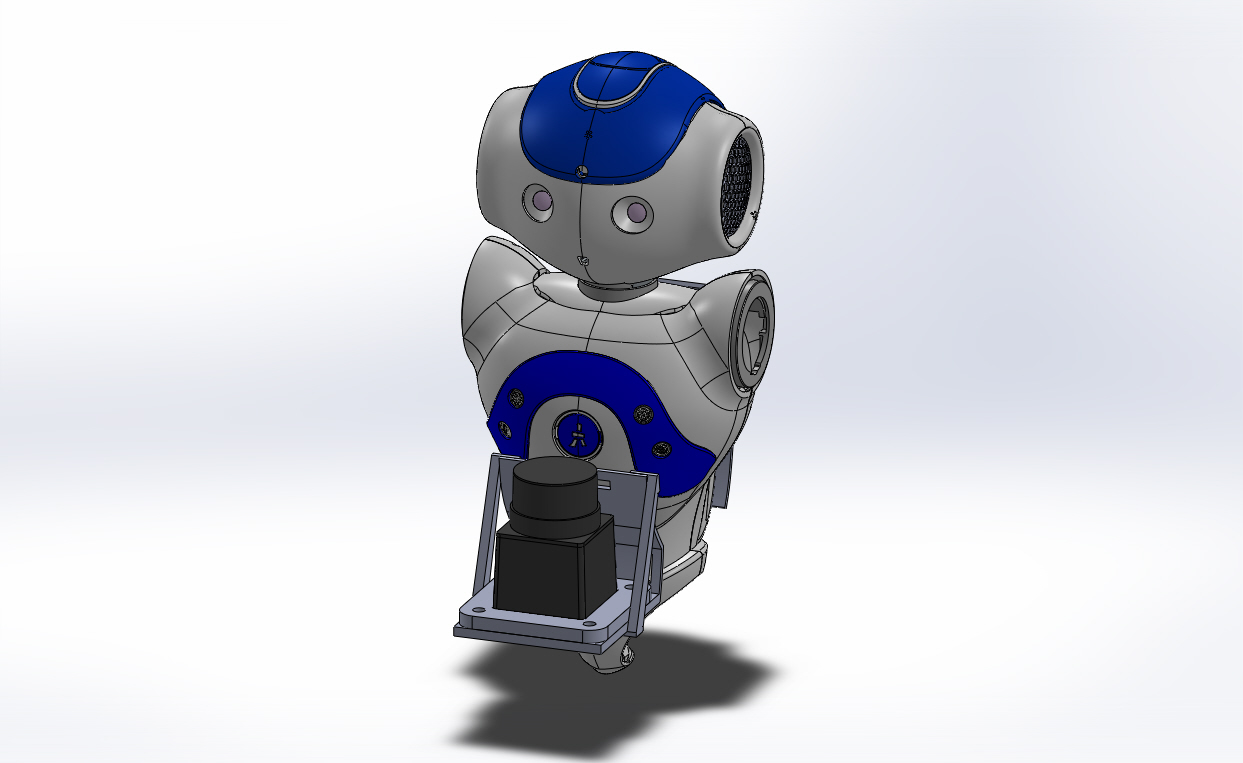
\includegraphics[height=0.4\textheight]{backpack/Assem_Nao_Dimetric1.jpg}
\caption{Figure showing CAD model of Nao with Hokuyo URG-04LX-UG01 mounted
         to the waist of the robot using a custom mount.}
\label{fig:nao_lidar_mount_nao_dimetric1}
\end{figure}

\begin{figure}
\centering
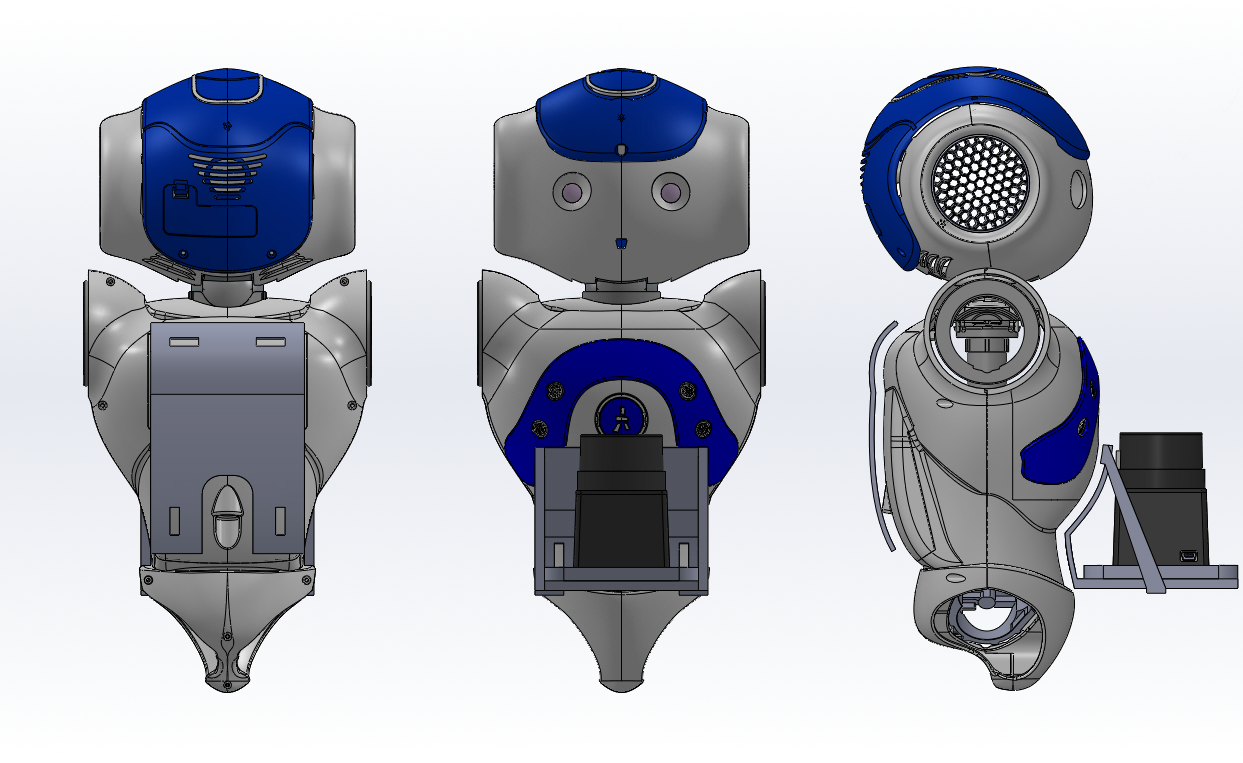
\includegraphics[height=0.4\textheight]{backpack/Assem_Nao_Three_View1.png}
\caption{Figure showing back, front, and side views of the URG CAD model 
         mounted to the Nao using the custom mount.}
\label{fig:nao_lidar_mount_nao_three_view1}
\end{figure}

The front subassembly of the Lidar mount consists of three parts: a front plate,
a base plate, and side supports. Figure~\ref{fig:nao_lidar_mount_dimetric1}
shows a CAD model of the assembled front subassembly with the URG installed.

\begin{figure}
\centering
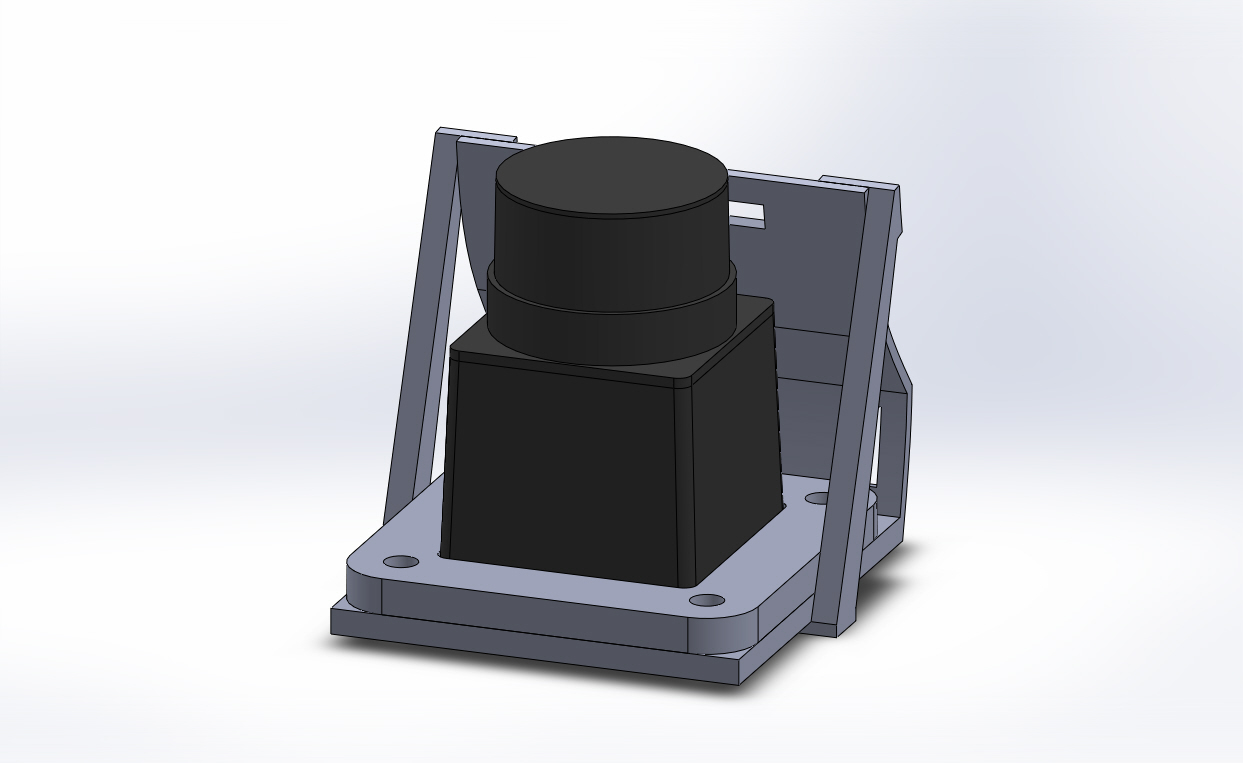
\includegraphics[height=0.4\textheight]{backpack/Assem_FrontOnly_Dimetric1.jpg}
\caption{Figure showing CAD model of the URG attached to the front subassembly
         of the custom Lidar mount.}
\label{fig:nao_lidar_mount_dimetric1}
\end{figure}

\begin{figure}
\centering
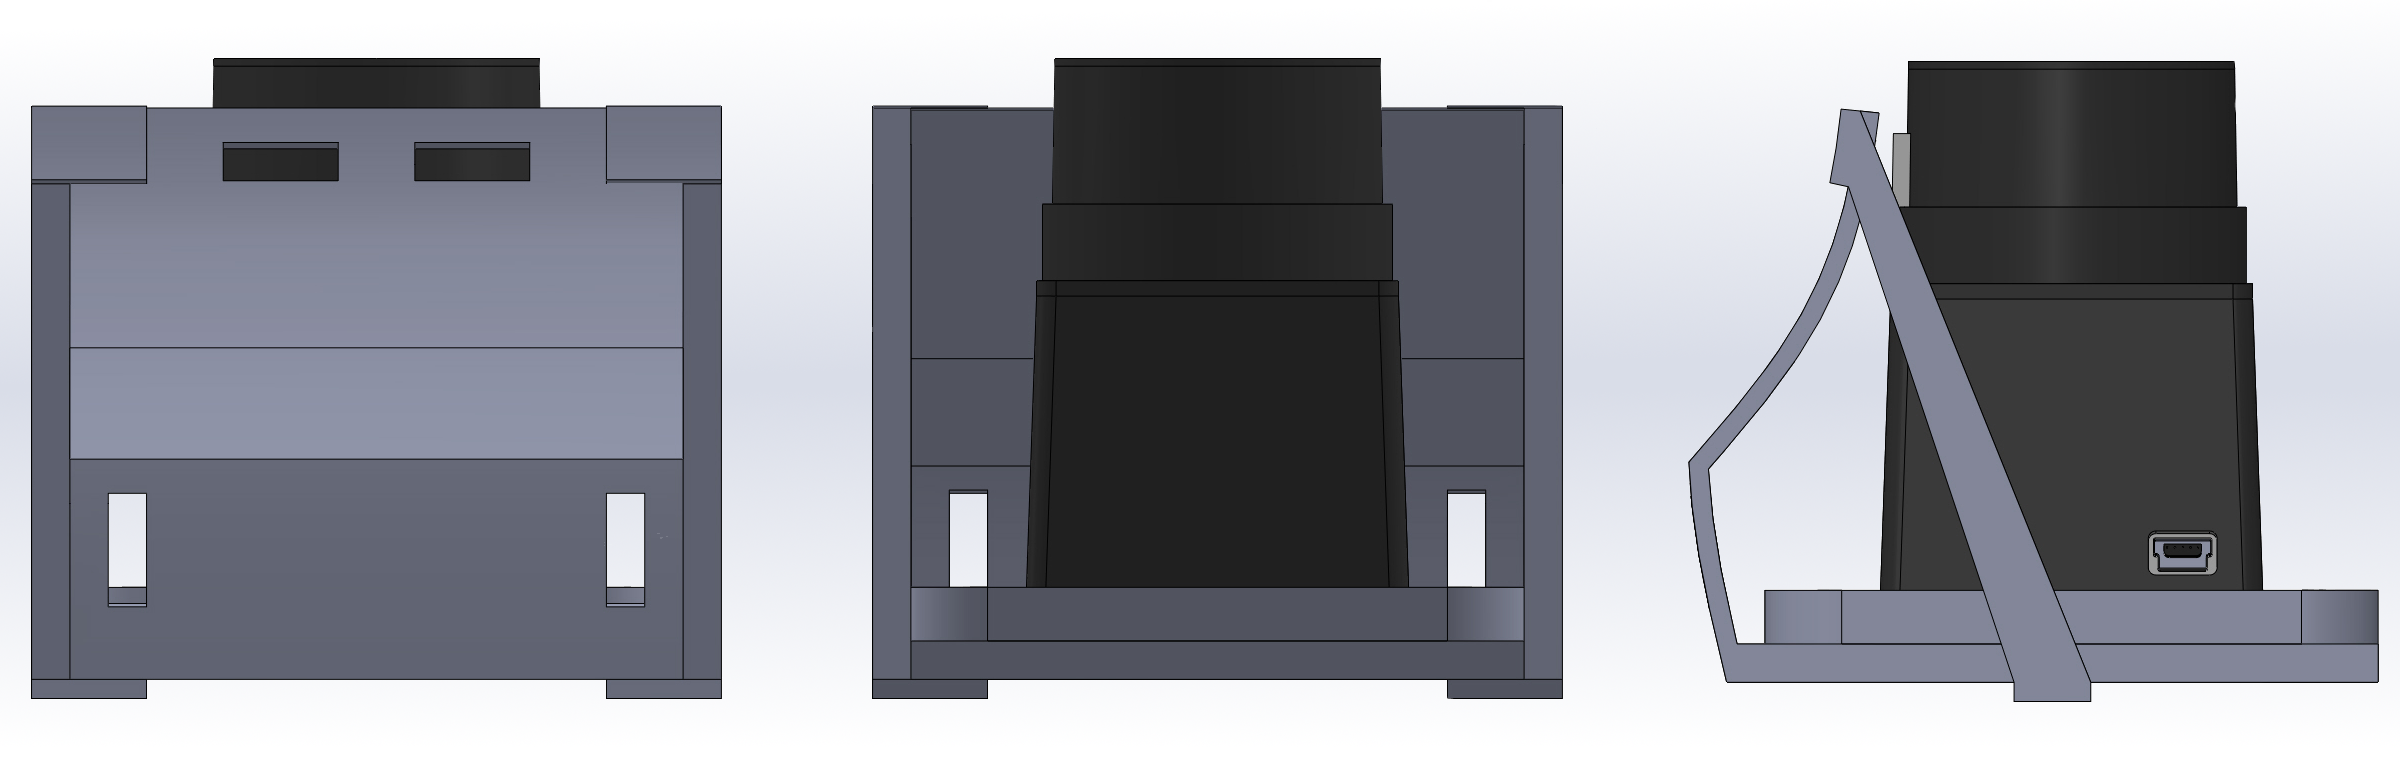
\includegraphics[width=\textwidth]{backpack/Assem_FrontOnly_Three_View1.png}
\caption{Figure showing back, front, and side views of the URG CAD model
         attached to the front subassembly of the custom mount.}
\label{fig:nao_lidar_mount_three_view1}
\end{figure}

The front plate has a shape that follows the form of the Nao.
It is padded with foam that is glued to the plate to conform to the robot more
closely and minimize the effects of vibration.
Figure~\ref{fig:nao_lidar_mount_frontplate_trimetric1} shows a CAD model of the
front plate. It has a tray that projects perpendicular from the robot to hold 
the base plate. Two mounting holes on the tray secure the base plate to the tray.
The front plate is secured to the robot via four rectangular holes which receive
velcro straps that go to the back plate. These straps are tightened to hold the
Lidar mount to the robot.

\begin{figure}
\centering
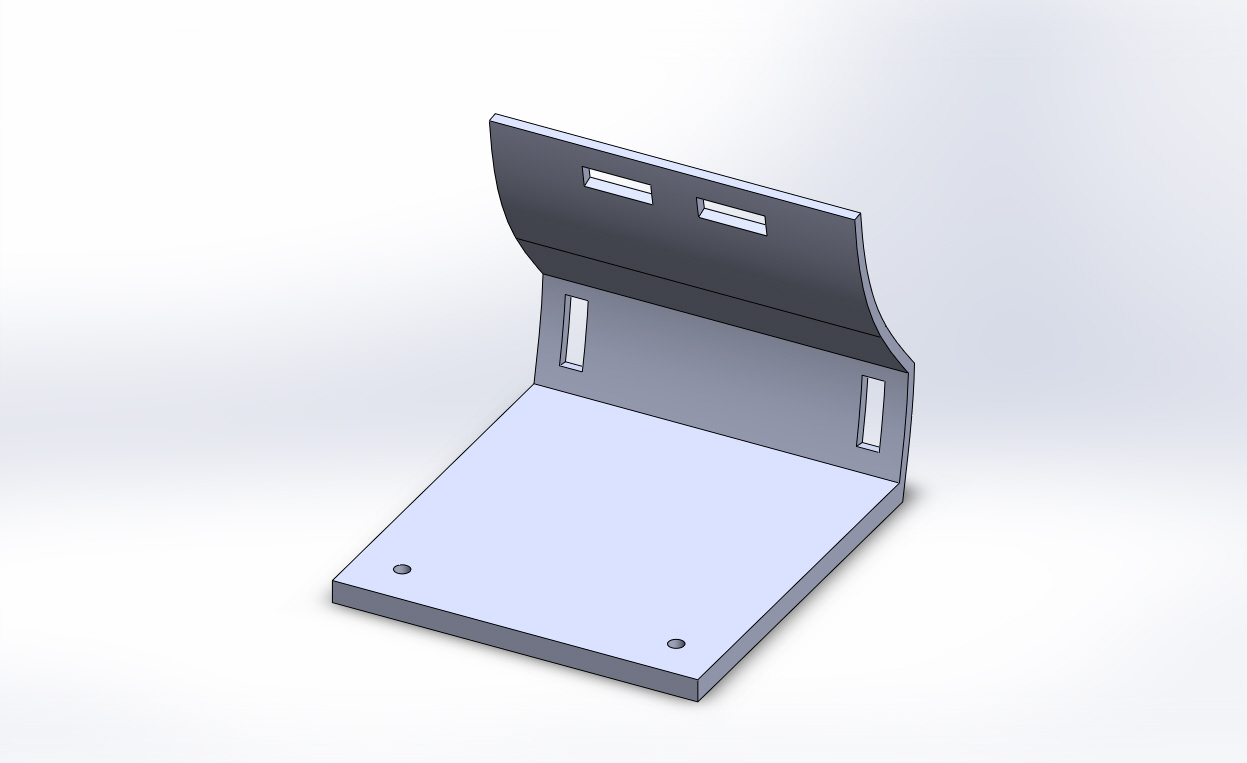
\includegraphics[height=0.4\textheight]{backpack/Front_Plate_Trimetric1.jpg}
\caption{Figure showing a CAD model of the front plate of the custom Lidar
         mount. The base plate attaches to this plate.}
\label{fig:nao_lidar_mount_frontplate_trimetric1}
\end{figure}

\begin{figure}
\centering
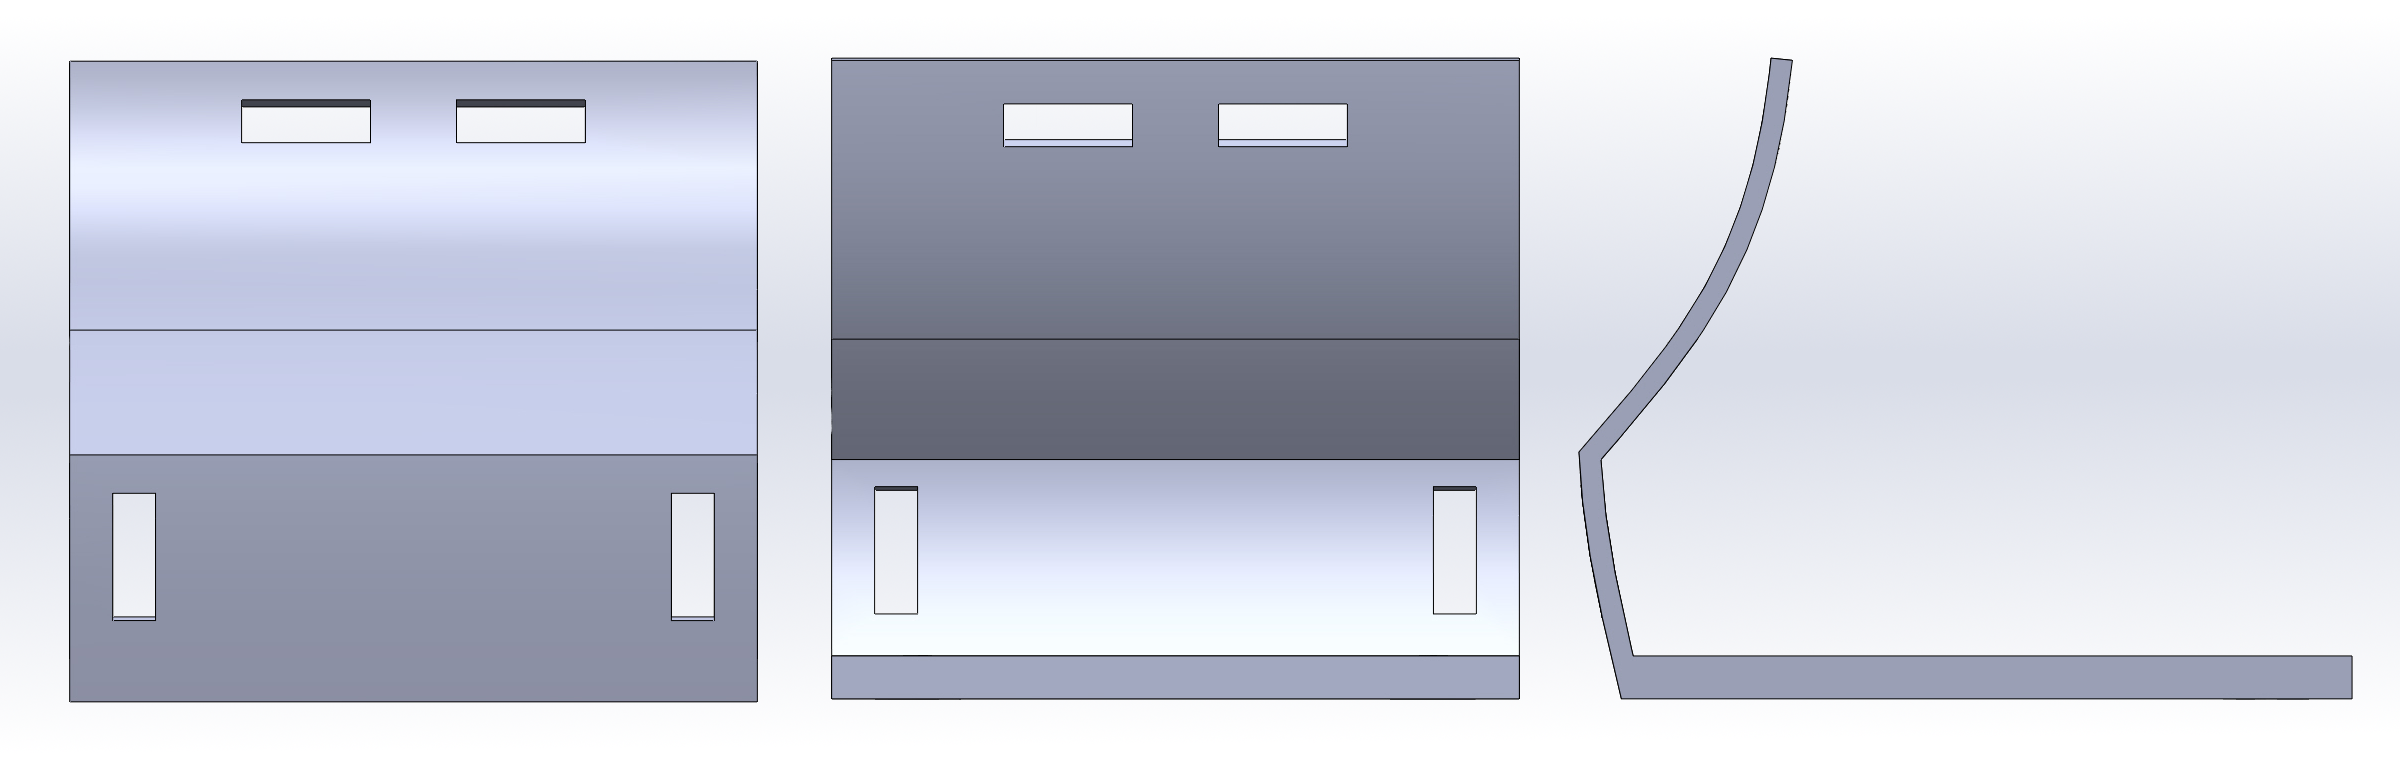
\includegraphics[width=\textwidth]{backpack/Front_Plate_Three_View1.png}
\caption{Figure showing back, front, and side views of the CAD model of the
         front plate.}
\label{fig:nao_lidar_mount_frontplate_three_view1}
\end{figure}

The URG is attached to the base plate, which in turn is attached to the 
tray of the front plate. The URG is attached to this intermediate part
rather than directly to the front plate to facilitate the mechanical
interoperability of different sensors to the front plate without needing
to produce different front plates for different sensors. Instead, different
base plates are made for different sensors. For example, the lower cost
RPLidar \cite{rp_lidar} or the VLP-16 Puck 3D Lidar
\cite{puck_lidar} are alternative Lidars that could
be mounted to the Nao for experimentation but have a different mounting 
configuration than the URG\@. In this way, new base plates can be manufactured
rather than front plates, allowing for a more modular design.

\begin{figure}
\centering
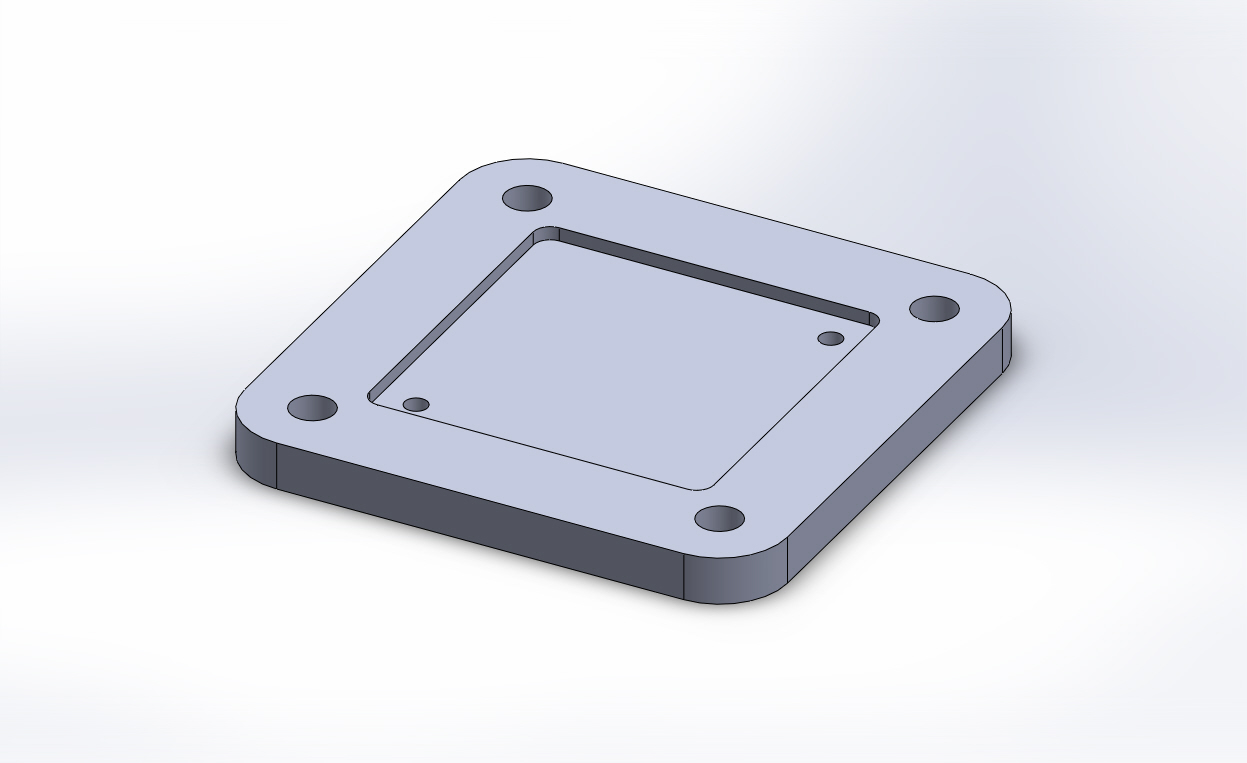
\includegraphics[height=0.4\textheight]{backpack/Base_Plate_Trimetric1.jpg}
\caption{Figure showing a CAD model of the base plate of the custom Lidar
         mount. The base plate is part of the front subassembly.
         The URG attaches to this plate.}
\label{fig:nao_lidar_mount_baseplate_trimetric1}
\end{figure}

\begin{figure}
\centering
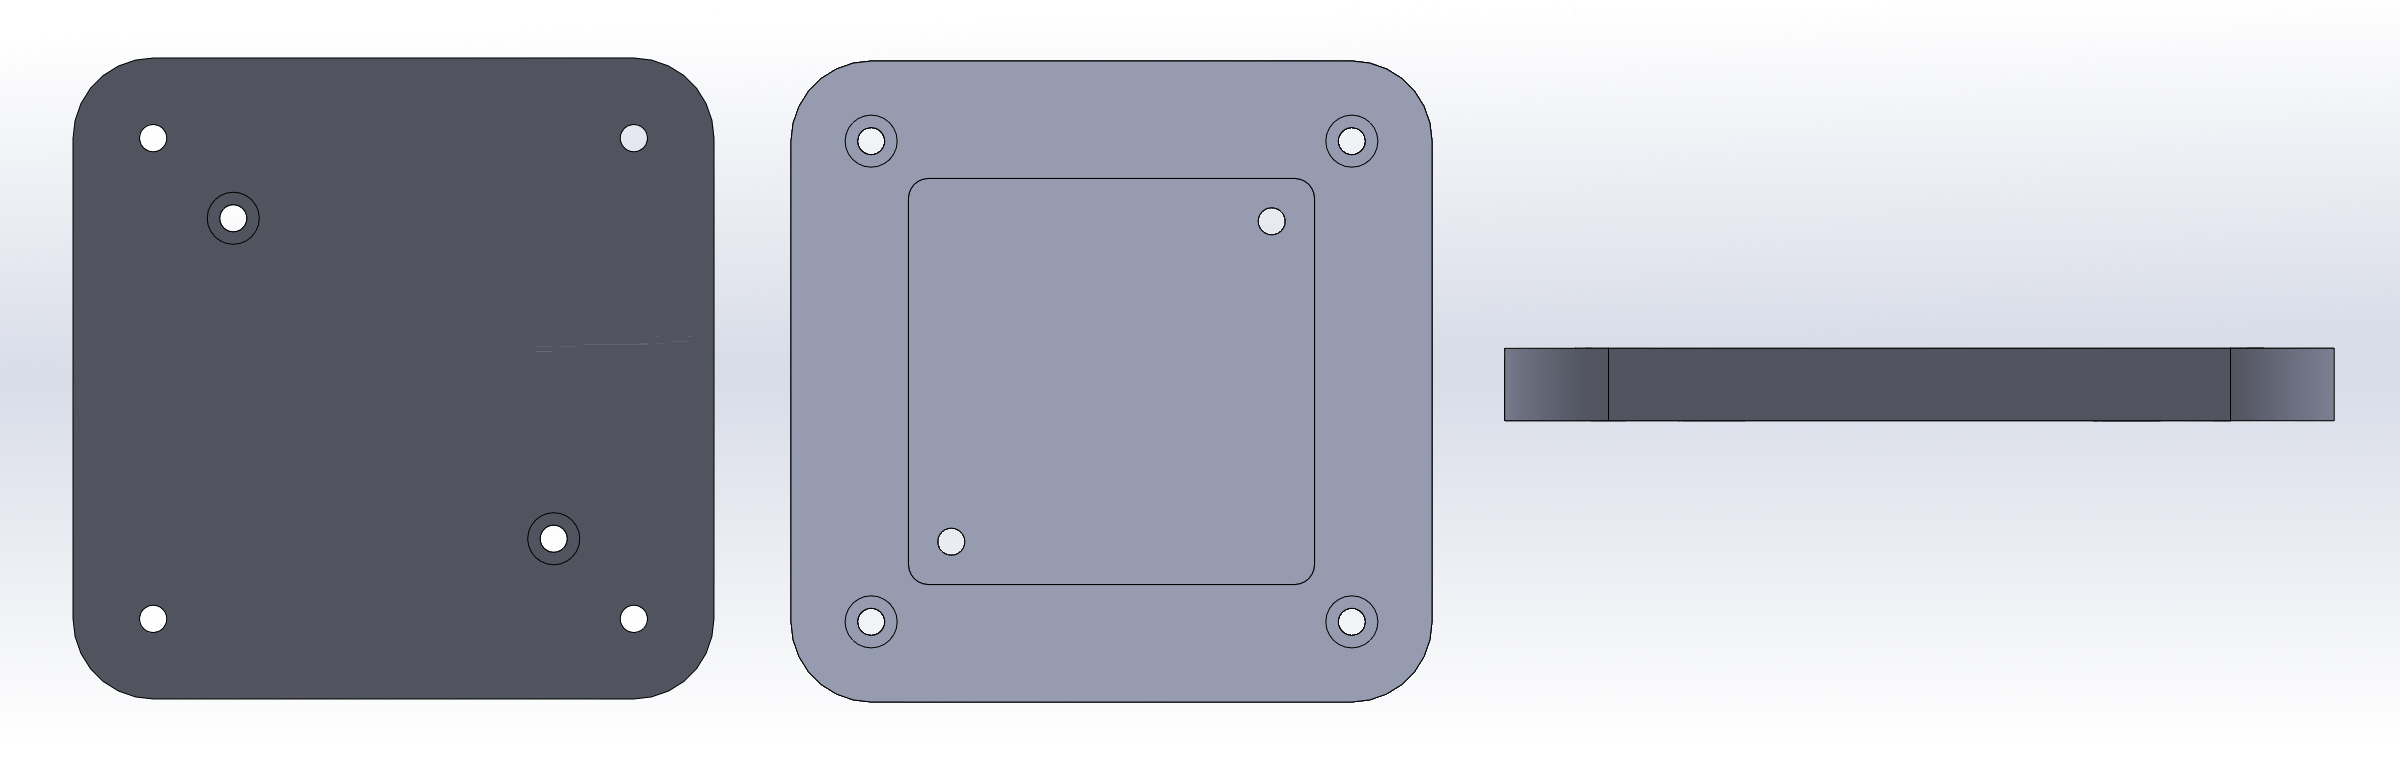
\includegraphics[width=\textwidth]{backpack/Base_Plate_Three_View1.png}
\caption{Figure showing back, front, and side views of the CAD model of the
         base plate.}
\label{fig:nao_lidar_mount_baseplate_three_view1}
\end{figure}

\begin{figure}
\centering
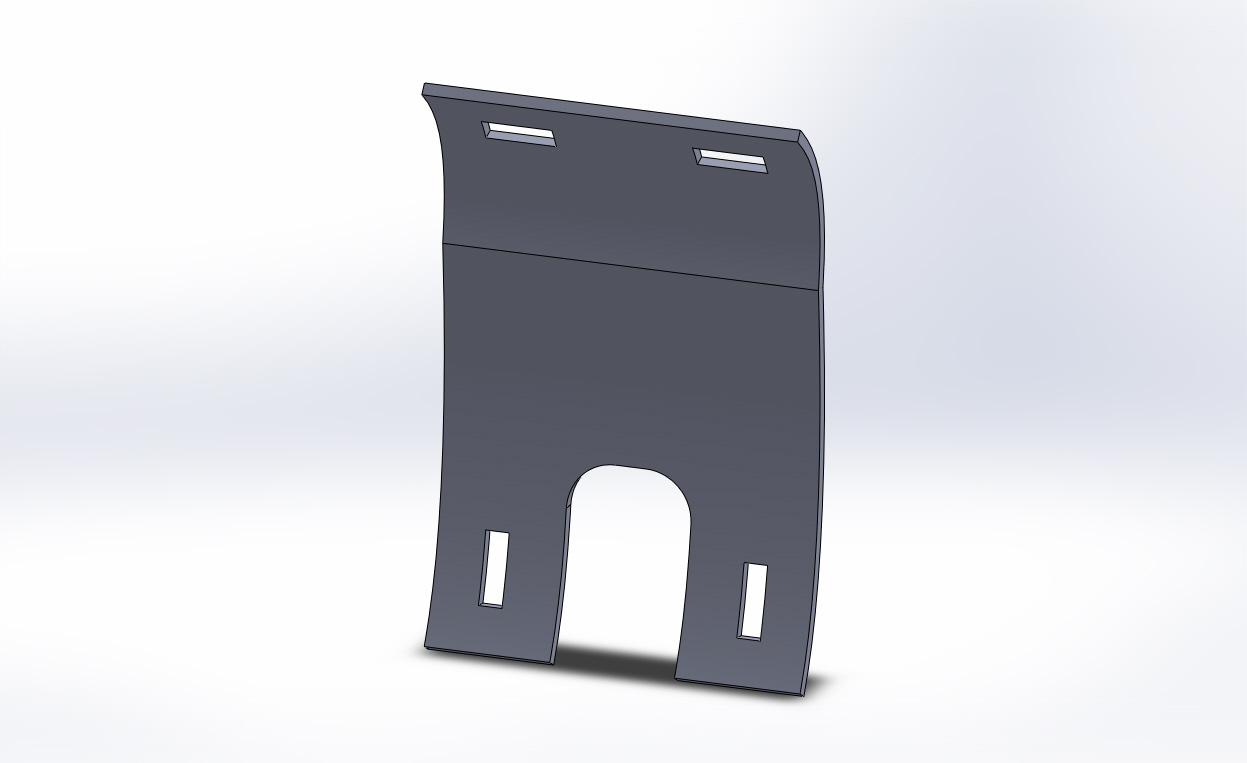
\includegraphics[height=0.4\textheight]{backpack/Back_Plate_Dimetric1.jpg}
\caption{Figure showing a CAD model of the back plate of the custom
         Lidar mount.}
\label{fig:nao_lidar_mount_backplate_dimetric1}
\end{figure}

\begin{figure}
\centering
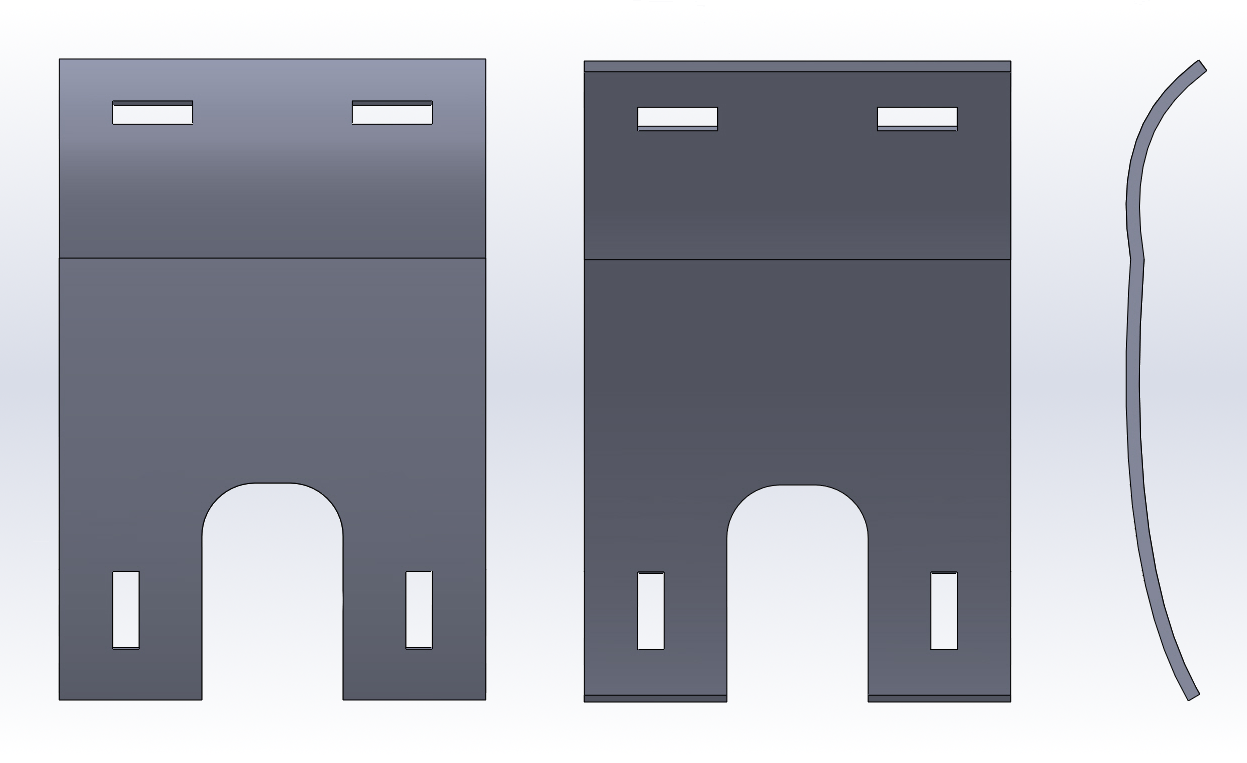
\includegraphics[width=\textwidth]{backpack/Back_Plate_Three_View1.png}
\caption{Figure showing back, front, and side views of the CAD model of the
         back plate of the custom Lidar mount.}
\label{fig:nao_lidar_mount_backplate_three_view1}
\end{figure}



\begin{figure}
\centering
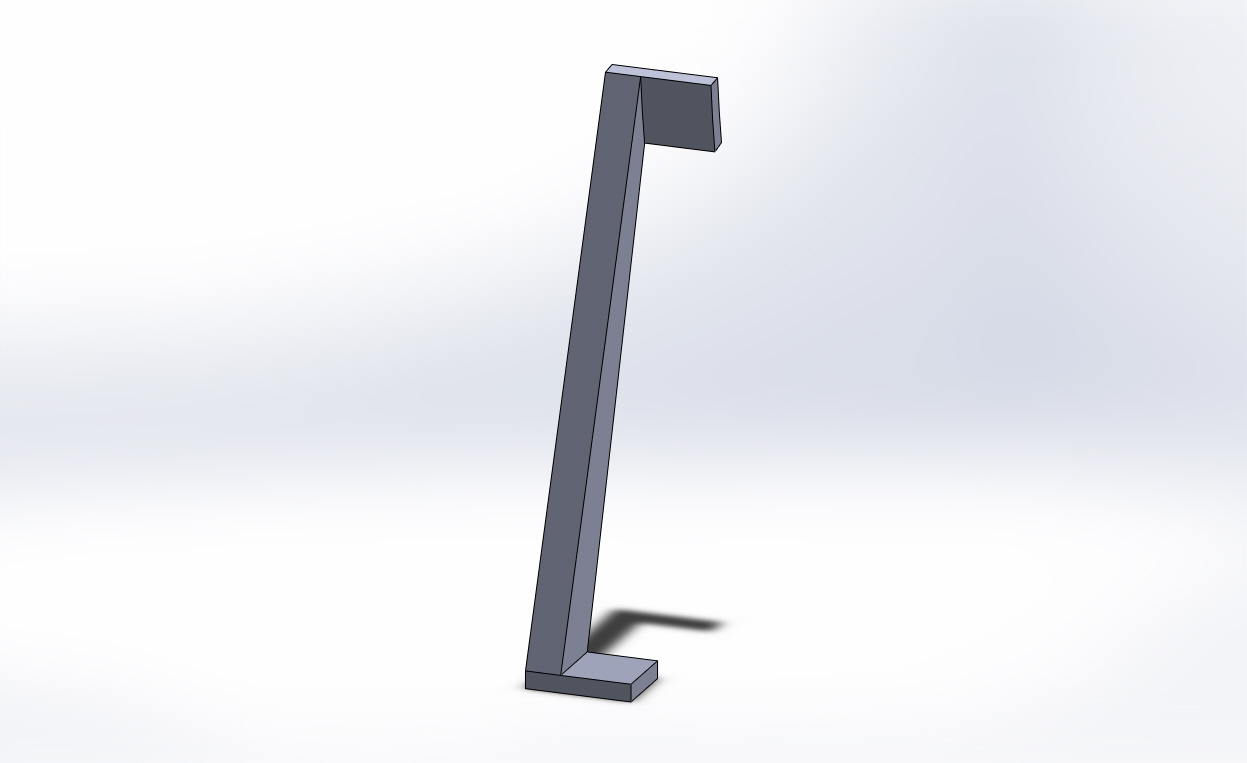
\includegraphics[height=0.4\textheight]{backpack/Support_Left_Trimetric1.jpg}
\caption{Figure showing a CAD model of the left side support of the custom
         Lidar mount. This support is bonded to the front plate to add rigidity
         to the front plate. The right side support is a mirror image of this
         part.}
\label{fig:nao_lidar_mount_supportleft_trimetric1}
\end{figure}

\begin{figure}
\centering

\includegraphics[height=0.4\textheight]{backpack/Support_Left_Three_View1.jpg}
\caption{Figure showing back, front and side views of the CAD model of the left
         side support.}
\label{fig:nao_lidar_mount_supportleft_three_view1}
\end{figure}


% Need some sort of System or summary Section.
